\newcommand{\defeq}{\buildrel {\text{ def }}\over =}
\newcommand{\leftrightarrowtriangleqrel}{\mathrel{\overset\triangleq\leftrightarrow}}

\startchapter{A Prediction Model}
\label{chap:predictionModel}
\section{Motivation}
As discussed in Chapter~\ref{chapter:introduction}, the main objective of this work is to increase the reliability of power networks in terms of power quality within given financial budget/resources. In order to monitor the power quality, power quality meters are being deployed. Since power quality meters are expensive devices, we (in Chapter~\ref{chap:PQEstimation}) proposed MaxEnt-based algorithm for power quality estimation on unmonitored network segments. For meter placements, we proposed conditional entropy-based efficient algorithms (in Chapter~\ref{chap:meterPlacement}) that intelligently place power meters on selected network segments so that the power quality could be inferred as accurately as possible.

Since the power quality readings (exact readings from monitored links, and estimated PQ values from unmonitored links) are available now, we use these readings to estimate the state of the network and identify any potential malfunctioning device in the power network. Our objective in this chapter is to address the research challenge: \textit{how to detect a potential malfunction device in the power network based on available power quality readings}. In this chapter, we propose a measure that helps to detect the malfunction devices in the power network. The simulation results confirm that the proposed solution is efficient, and accurate.

\section{Problem Formulation}
In this section, first we detail our assumptions of the problem domain and then formulate our research problem.

\subsection{Assumptions}
The four assumptions we make about the problem are as follows:
\begin{enumerate}
\item \textbf{The transfer function or behavior $\left(f\left(d\right)\right)$ of each device $d$ in the network is known}. As discussed earlier, a device-specific power quality transfer function could be estimated through physical modeling or through the assessment of historical PQ data. In Chapter~\ref{chap:latentF}, using our real power quality dataset, we have demonstrated that how accurately the transfer function $f(d)$ could be estimated.

\item \textbf{All potential malfunction devices need to be on a monitored segment.} A potential malfunction device could effectively be detected when the device itself or any of its child device is monitored in real time using a PQ meter. This assumption is realistic in the sense that if the underline link is not monitored, we cannot get the real-time status of PQ values and would not be able to detect if a device is not behaving normally. On a monitored segment, the objective is to detect a device as a malfunction when that is significantly deviating form its normal behavior by producing bad power quality.

\item \textbf{The power grid network is a tree-structured network where the electric current flows from root node to the child nodes.} As discussed in Chapter~\ref{chap:meterPlacement}, this is a reasonable assumption at any particular instance in time. While enterprise-level power grids used in places such as hospitals and data centers often have two utility feeds available as well as an independent emergency power source, only one power source is typically used at one time. See the IEEE Gold Book~\cite{goldbook} for further information on recommended practices in the design of critical power systems.

\item \textbf{The probability mass function $(f_x\left(d_0\right))$ of power quality values at the input link to the root node is known.} In other words, the distribution of power quality at the input to the network, usually the utility feed, is known. This is also a reasonable assumption, since electrical utilities typically report on indices such as System Average RMS Variation Frequency Index (SARFI) which is essentially a count of the number of times the magnitude and duration falls below a threshold. Furthermore, there are often independent bodies that gather statistics on power delivery service reliability that can also be incorporated into an estimate of power quality distribution~\cite{chowdhury2004reliability}.
\end{enumerate}


\begin{figure}[!p]
\centering
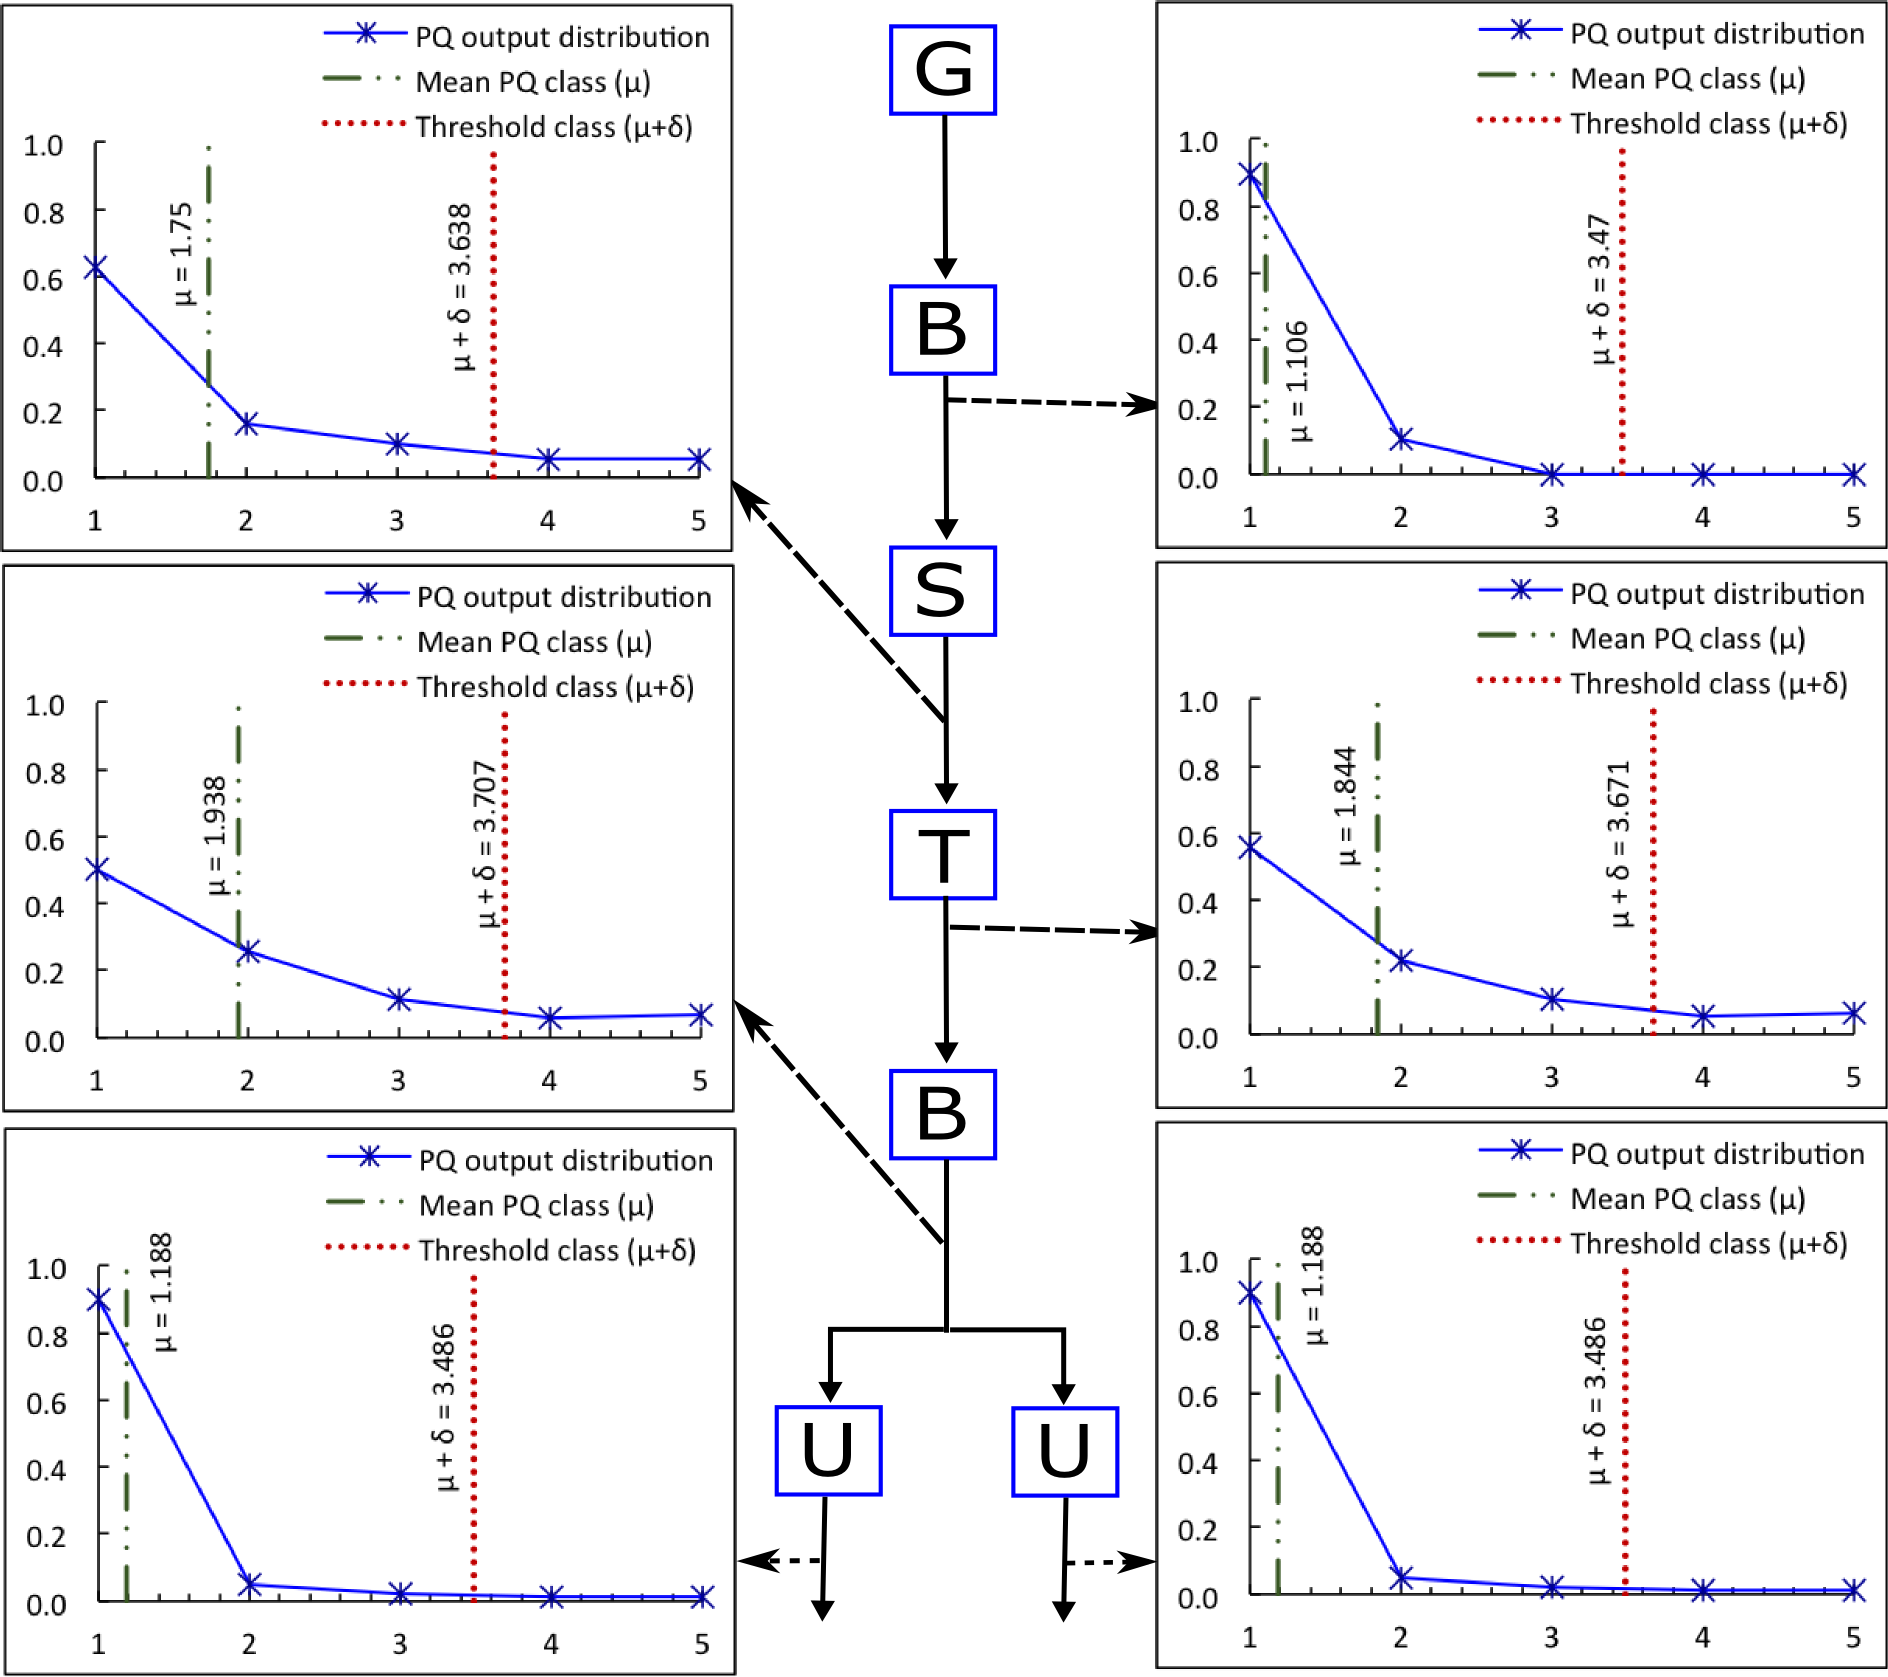
\includegraphics[width=0.98\textwidth]{PQOutputDistribution} \vspace{1cm}
\caption{Power quality distributions and their average output power quality class for various devices. The average power quality class and computed threshold is shown as vertical lines in each  distribution graph. The x-axis represents the power quality class $c_i$ while the y-axis represents the probability of $c_i$. Further, the lower class $c_1$ represents the best power quality while $c_5$ represents the worst power quality.}
\label{fig:outputPQDistributions}
\end{figure}

\subsection{The Problem}
We now formulate the problem of detecting a malfunction device in the network. The objective is to detect a device $d$ in the network as a malfunction device when its power quality output degrades persistently from its normal/actual behavior. Since the transition function $f(d)$ of each device $d$ is known, we know the probability distribution of the output power quality ($f_x\left(d\right)$) at the output link of each device in the power grid network. Figure~\ref{fig:outputPQDistributions} shows the probability distributions for various devices in a sample network. The distributions are obtained/computed for the prior distribution of$\begin{array}{ccccc}[0.9947 & 0.005 & 0.0002 & 0.00009 & 0.00001]\end{array}$at the utility feed/generator.

We mathematically analyze these distributions and based on their various statistical properties, we propose out detection algorithm in the next section. The proposed algorithm compares the normal behavior ($f_x\left(d\right)$) of each device with the observed behavior ($\overset{\circ}{f_x}\left(d\right)$) and compute the power quality degradation (the difference between the two distributions) as $\Delta_d$ . The objective function becomes:

\begin{equation}
\label{eq:pqPrediction}
\Delta_d = f_x\left(d\right) \leftrightarrowtriangleqrel \overset{\circ}{f_x}\left(d\right)
\end{equation}

\noindent where the operation $\leftrightarrowtriangleqrel$ is unknown. In the next section,  we propose algorithms to solve the Eq.~(\ref{eq:pqPrediction}).

\section{Our Detection Algorithms}
\subsection{A Simple Correlation Measure}
To compare two probability distributions, the correlation measure is usually used where its most familiar type is the \textit{Pearson's correlation coefficient}, simply known as \textit{the correlation coefficient}. In order to use the formula, we represent the actual PQ distribution as X while the obtained distribution as Y. For the random variables X and Y, it is defined as:
\[\rho_{X,Y} = corr(X,Y) = \frac{\sum (x-\bar x) (y-\bar y)}{\sqrt{\sum (x-\bar x)^2 \sum (y-\bar y)^2}}\]

The above correlation measure could be used to compare the actual and observed PQ distributions. Generally speaking, this measure can accurately tell how much the observed distribution is similar to (or different from) the actual distribution of the same device. When a device is perfectly behaving like its actual distribution, the measure returns a maximum value (  +1). On the other hand, when a device is producing a very different distribution (for instance producing very bad PQ), it returns a smaller value (the smallest possible is -1). The value 0 (or closer to 0) represents that the two distributions have no correlation, i.e., they are asymmetric. Although this technique is simple to use, there are certain assumptions to be true in order to effectively use it. These assumptions include: related pairs, absence of outliers, normality of variables, and linearity. These assumptions may not always be true and hence we cannot use this measure as a complete solution.

We demonstrate various scenarios where the above correlation assumptions do not hold and hence we cannot effectively use it to accurately detect a malfunction device in the power network. We classify the identified scenarios in two classes: 1) a malfunction device is not detected; and 2) a better PQ producing device is classified as a malfunction. Both cases are explained as follows.

\begin{figure}[!p]
\centering
\subfloat[Positive correlation ($\rho_{X,Y} = +0.95 \approx +1$)]{\label{corr_positive}
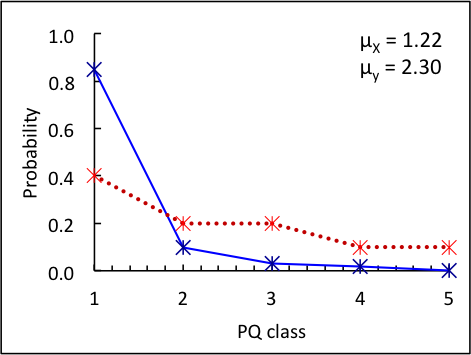
\includegraphics[width=0.6\columnwidth]{corr_positive}
}

\vspace{1cm}

\subfloat[Zero correlation ($\rho_{X,Y} = 0$)]{\label{corr_zero}
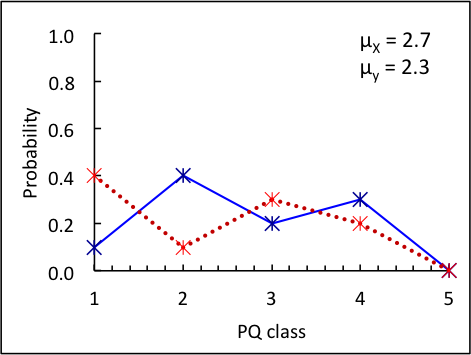
\includegraphics[width=0.6\columnwidth]{corr_zero}
}
\vspace{0.5cm}
\caption{Positive correlation scenarios where the simple correlation technique is not useful.} 
\vspace{1cm}
\label{correlationAnalysisPositive}
%\vspace{-0.15in}
\end{figure}


\begin{figure}[!p]
\centering
\subfloat[Negative correlation ($\rho_{X,Y} = -1$)]{\label{corr_negative_low}
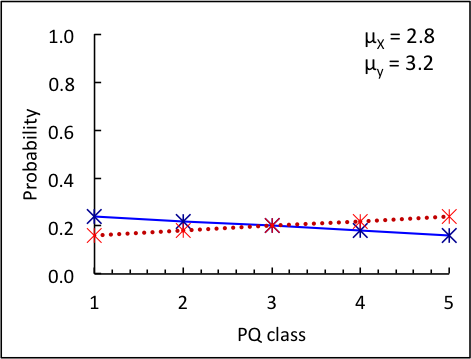
\includegraphics[width=0.6\columnwidth]{corr_negative_low}
}

\vspace{1cm}

\subfloat[Negative correlation ($\rho_{X,Y} = -1$)]{\label{corr_negative_high}
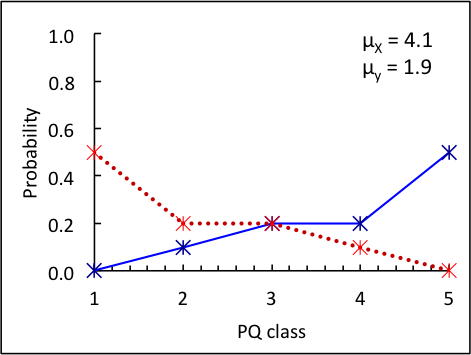
\includegraphics[width=0.6\columnwidth]{corr_negative_high}
}
\vspace{0.5cm}
\caption{Negative correlation scenarios where the simple correlation technique is not useful.} 
\vspace{01cm}
\label{correlationAnalysisNegative}
%\vspace{-0.15in}
\end{figure}

\subsubsection{Missed Detection Scenarios}
This scenario arises when a device is producing a very bad power quality (malfunction device) and the system does not detect it. This measure classifies the observed distribution as perfectly normal (similar to the actual) when the correlation is a +1 (or close to +1). For all normal behaving devices, the observed distribution will be very similar to the actual and a +1 correlation will perfectly classifying them as normal. Nevertheless, we identified cases where the PQ is significantly degraded and the distributions were still highly correlated. In all those cases, we cannot use this simple correlation measure. Figure~\ref{corr_positive} shows one such example where the power quality is significantly degraded (the dotted line) and the correlation coefficient is still very high (a +1).

\subsubsection{False Detection Scenarios}
We call it a false detection when a device that is generating similar or slightly different (good or bad) power quality output than its normal and classified as a malfunction. Using the correlation measure, a device is detected as malfunction when the correlation coefficient is negative or (closer to 0). Although we observed that this measure works in various cases, we have been able to identify few scenarios where the simple correlation measure will not work. These scenarios are explained under two categories as follows:

\begin{enumerate}
\item \textbf{Zero correlation:} A zero correlation means the two distributions do not share any particular correlation. In our case, most probably, observing a distribution which do not share any correlation with its actual distribution implies the degradation in the power quality. Nevertheless, based on the correlation measure only, we cannot tell for sure if the observed (and non-correlated) distribution is better or worse than its actual distribution in terms of power quality. Figure~\ref{corr_zero} represents a scenario where the observed power quality is better than its actual expected behavior. In such cases, simply based on a zero correlation, we cannot classify those devices as malfunction.

\item \textbf{Negative correlation:} In a negative correlation between two variables, the value of one variable increases when the other decreases, and vice versa. Although theoretically possible, it is rare to get a perfectly negative correlation in power quality measures. In a negative correlation, the observed distribution is either bad or good compared to the actual distribution. Although the probability of getting a bad PQ is higher than that of a good, it cannot always be guaranteed. Further, the negative correlation can quantify the symmetry of two distributions, it cannot essentially quantify how much the distributions are different in terms of power quality degradation. For instance, Figure~\ref{corr_negative_low} shows a 100\% negative correlation (with coefficient of -1) but the actual PQ degradation is very minor. Finally, as another evidence, we in Figure~\ref{corr_negative_high} demonstrates a significant PQ improvement with a correlation of -1.

\end{enumerate}

\begin{figure}[!p]
\centering
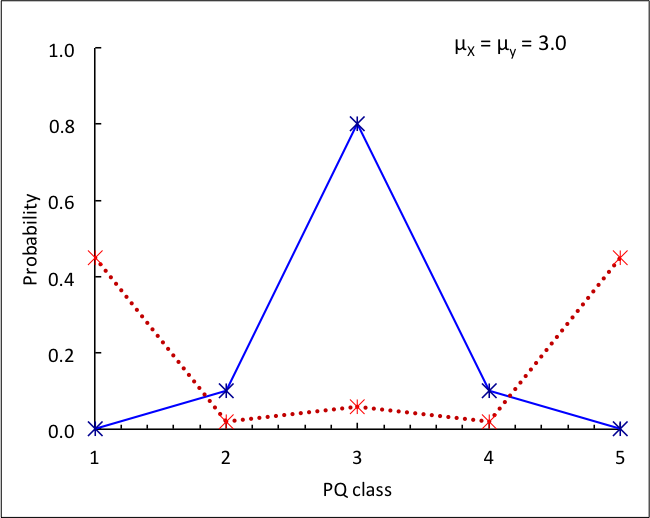
\includegraphics[width=0.6\textwidth]{average_pq_exception}
\vspace{1cm}
\caption{Two very different power quality distributions with same expected/average PQ output/class.}
\vspace{2cm}
\label{fig:average_pq_exception}
\end{figure}

\subsection{An Expected Value-based PQ Measure}
This measure is based on measuring the average power quality output over a period. A device is classified as a malfunction if its observed PQ output significantly degrades from its actual average power quality output. Clearly, if a device starts to malfunction by producing bad PQ output, its average output will deviate from its actual average output. We measure this deviation as $\Delta_d$ and is computed as follows.

\[\Delta_d = E[f_x(d)] - E[\overset{\circ}{f_x}(d)] \leq \theta_d \]

\noindent where $\theta_d$ is the threshold/maximum value allowed at which a device is classified as malfunction. In other words, $\theta_d$ is the maximum allowed deviation between the expected PQ classes of the two distributions. The value of $\theta_d$ could be fixed for all devices. For instance, by using $\theta_d = 1$, any device whose average output degrades by 1 PQ class from its actual average output will be classified as a malfunction device. We use $\theta_d$ equal to the standard deviation of the actual output distribution, i.e., $\theta_d=\sigma_d$. Using standard deviation as threshold will allow us to use slightly larger/relaxed threshold for devices generating less uncertain outputs in normal conditions (compared to other devices in the same network). Figure~\ref{fig:outputPQDistributions} shows the expected value and corresponding threshold values for various devices in our sample power grid.

The proposed measure is simple and accurately detects malfunction devices in the network. On the contrary, it is theoretically possible to produce two very different PQ distributions with same average/expected value. One such scenario is demonstrated in Figure~\ref{fig:average_pq_exception} where two very different power quality output distributions have exact same expected output PQ class. Since, on average, the two distributions in Figure ~\ref{fig:average_pq_exception} represents the same power quality, it is debatable whether the observed distribution is better or worse than its normal. We take a safer approach and address the problem by proposing a composite measure as follows.

\subsection{A Composite Measure}
As discussed earlier, we know that the average power quality degrades (to a higher PQ class) when a devices produce significantly bad power quality than its actual power quality. Simply measuring the difference between the expected values of the actual, and observed PQ classes can accurately detect a malfunction device. Although this simple technique works well, theoretically it is possible that a very different observed PQ output may produce similar expected values. To address this problem, we propose a composite expected value measure that enhances the accuracy of detecting a malfunction device in terms of power quality degradation.

\begin{algorithm}[!p]
\setstretch{1.5}
\vspace{0.3cm}
\KwIn{distribution function of input link to device 1 i.e., $f_x(0)$, transfer function $f(d)$, network topology $T$, set of positions of the installed power meters $M$}
\KwOut{$L$ (list of devices detected as malfunction)}
\Begin{
 \BlankLine
/* One time parameter computations */\\
 \ForEach {(Device $d$ in level order)}{
    $parent \leftarrow$ getParent($d$);  $f_x(d) \leftarrow f_x(parent) \times f(d)$; \\
    $\mu_f^d \leftarrow$ computeFullMean($f_x(d)$);  $\mu_p^d \leftarrow$ computePartialMean($f_x(d), \mu_f^d$); \\
    $\sigma_f^d \leftarrow$ computeFullSDev($f_x(d)$);  $\sigma_p^d \leftarrow$ computePartialSDev($f_x(d), \mu_f^d$);\\
 } 
 \BlankLine
 
 
 \BlankLine 
 
 /* Every meter records a PQ events $e_d^{(t)}$ continuously (usually every few seconds) \\ 
 $e_d = [e_d^{(1)}, e_d^{(2)}, \hdots, e_d^{(w)}]$ is the set of PQ recordings for a metered device $d$ */ \\
\ForEach {(Time Interval $t$)}{
   \ForEach{(Metered Device $d$)}{
      /* get latest W readings for each metered device $d$ */ \\
      $e_d \leftarrow$ getLastestReadings($w,d$);\\
      $\mu_F \leftarrow$ computeFullMean($e_d$);\\
      $\mu_P \leftarrow$ computePartialMean($e_d$, $\mu_f^d$);\\
      \If{($(\mu_F - \mu_f^d) > \sigma_f^d\ ||\ (\mu_p - \mu_p^d) > \sigma_p^d$)}{
         $L$.add($d$);      
      }
    }
   }
}
\caption{A malfunction device detection algorithm} \label{algo:malfunDetectionAlgo}
\end{algorithm}

In the composite expected value measure, we calculate two different expected values: 1) expected value of the complete distribution; and 2) expected value of the PQ classes greater than the average class computed on complete distribution (all classes). This composite measure increases the accuracy of our detection solution. In other words, for a malfunction device, if the observed expected value is similar to the actual expected value, the probability values of the higher classes must be greater (or the device is not a malfunction). Our proposed algorithm is shown as Algorithm~\ref{algo:malfunDetectionAlgo}. The main steps in the algorithms are described as follows.

\begin{enumerate}
\item \textbf{Input parameters:} The proposed algorithm requires these parameters: 1) network topology, 2) metered locations, 3) device transfer functions $f(d)$, 4) prior distributions $f_x(d_0)$, and 5) size of the sliding size $w$ that represents the number of PQ readings to use for computing our composite measure. Further, we compute the actual standard deviation of each device $\sigma_d$ from the actual output distributions.
\item \textbf{PQ readings from metered locations:} The installed power quality meters measure send the power quality reading to a central location. Our algorithm continuously reads these recordings/readings.
\item \textbf{Computing $\Delta_d$:} In order to compute the $\Delta_d$, we need the actual and observed expected values. The expected values of the actual distributions are computed only once while while the observed values are computed periodically using new PQ reading in that interval.
\item \textbf{Device classification:} Periodically after a fixed interval $t$, the algorithm compares the observed expected values (both and full partial) and classifies a device $d$ as malfunction if any of the observed measures exceeding by $\theta_d$ from its actual expected values.
\end{enumerate}


\section{Performance Evaluation}
\subsection{Simulation Setup}
We simulate the power grid network in MATLAB. The inputs include: 1) Network topology as an adjacency matrix, 2) device type (e.g., bus, switch, UPS, transformer etc) of each node, 3) transfer matrix $f(d)$ for each node $d$, 3) PQ distribution vector $f_x(d_0)$ of the utility feed, and 4) vector of metered locations.

The power quality events were generated using the input distribution $f_x(d_0)$, and transfer function $f(d)$ in level order starting from the root node of the tree. A power quality event $e_d$ at a node $d$ is generated based on the event at its parent link ($e_{\widehat d}$). For example a PQ event of class $c_3$ at a parent link will result into a child event following the distribution in $3^{rd}$ row of $f(d)$. Since the transfer matrices $f(d)$ are computed using our real PQ dataset (see Chapter~\ref{chap:latentF}), the simulated events possesses similar statistical features.

\begin{figure}[!p]
\centering
\subfloat[Homogenous line network]{\label{mf_line_homogeneous}
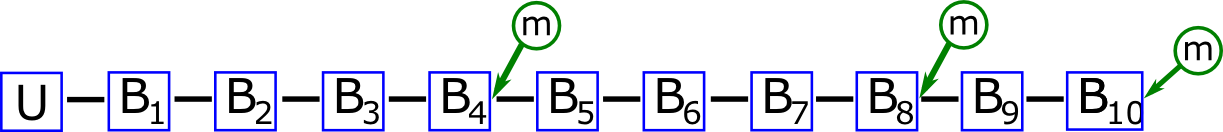
\includegraphics[width=0.78\columnwidth]{mf_line_homogeneous}
}

\begin{centering}
\subfloat[Heterogeneous line network]{\label{mf_line_heterogeneous}
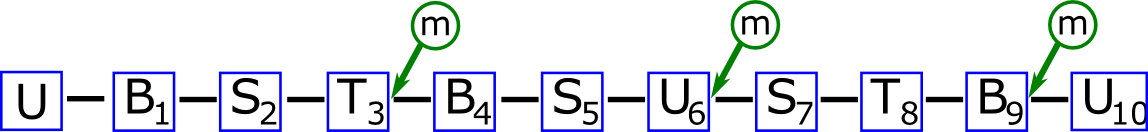
\includegraphics[width=0.75\columnwidth]{mf_line_heterogeneous}
}
\end{centering}

\begin{centering}
\subfloat[Heterogeneous tree network]{\label{mf_tree_heterogeneous}
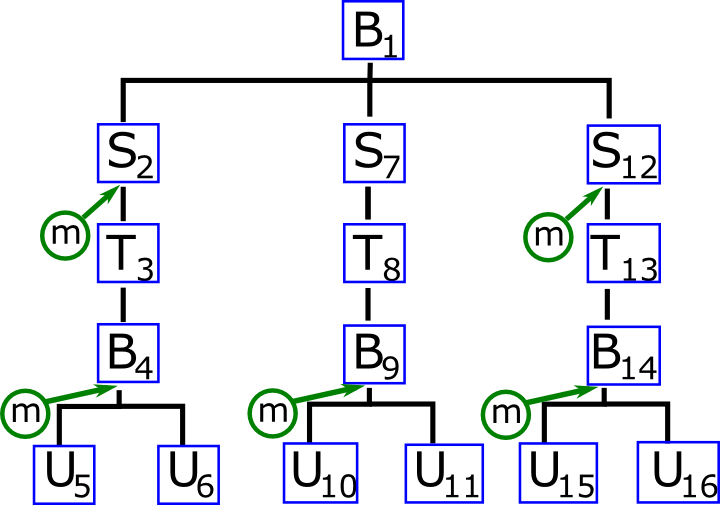
\includegraphics[width=0.5\columnwidth]{mf_tree_heterogeneous}
}
\end{centering}

\begin{centering}
\subfloat[IEEE 13-node distribution test feeder network]{\label{mf_IEEE_test_feeder}
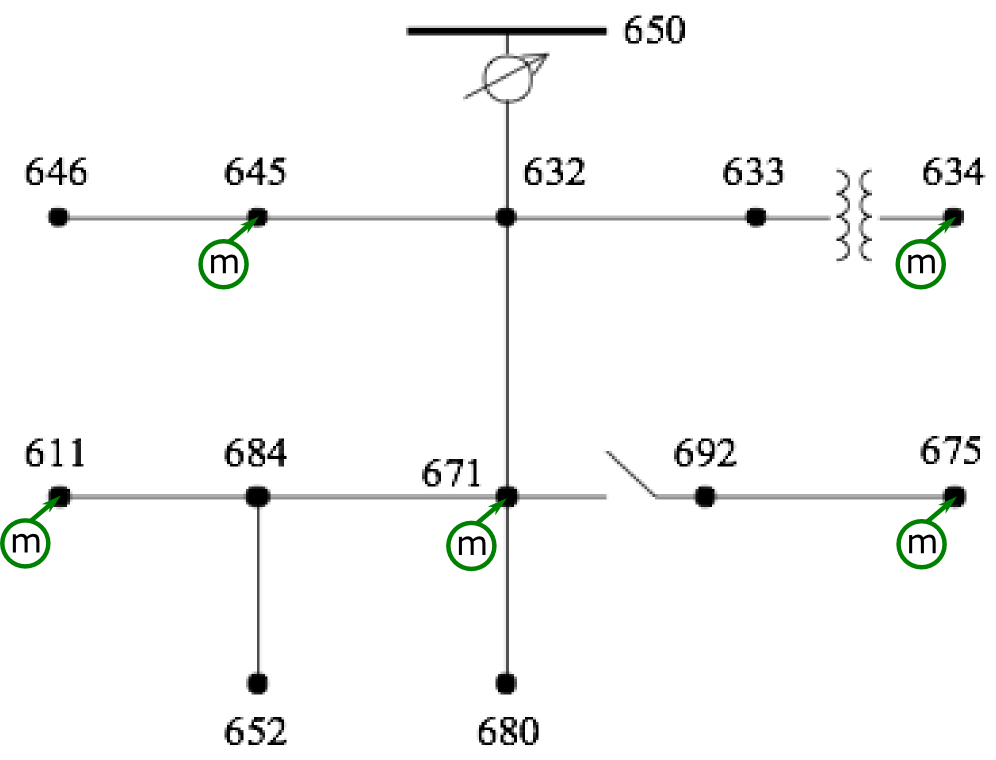
\includegraphics[width=0.6\columnwidth]{mf_IEEE_test_feeder}
}
\end{centering}
\vspace{0.5cm}
\caption{Networks used in our experiments. B=bus, S=switch, T=transformer,
U=UPS. The circled m indicates the position of a meter. The meter positions are based on our meter placement solution proposed in Chapter~\ref{chap:meterPlacement}.}
\vspace{1cm} 
\label{mf_networks_used}
\end{figure}

We select a device $d$ in the start of our simulation as a malfunction device and modify its transfer function from $f(d)$ to a malfunction transfer function $\acute f(d)$. The objective is to detect the effect of a malfunction device at the following metered location. The process was repeated for all devices by infecting one device at a time. For a malfunction device, we use a uniform transfer function, e.g., for five event types, the transfer function is

\[\acute f(d) = \left[\begin{array}{ccccc}
0.2 & 0.2 & 0.2 & 0.2 & 0.2\\
0.2 & 0.2 & 0.2 & 0.2 & 0.2\\
0.2 & 0.2 & 0.2 & 0.2 & 0.2\\
0.2 & 0.2 & 0.2 & 0.2 & 0.2\\
0.2 & 0.2 & 0.2 & 0.2 & 0.2\end{array}\right].\]

\noindent Experimental results on various network types are discussed next.

%In a malfunction $\acute f(d)$, the probability of generating a good power quality is reduced while the probability of generating bad power quality is increased. In our experiments, the changed in $\acute f(d)$ were: 1) decreased the probability of power quality classes $c_1$ and $c_2$ by 0.2; 2) $c_3$ were left unchanged, 3) $c_4$, and $c_5$ were increased by 0.2. 


\subsection{Simulation Results}
Figure~\ref{mf_networks_used} show various network types used in our simulation to evaluate the accuracy of our proposed solution. The metered position are obtained using our meter placement solution from Chapter~\ref{chap:meterPlacement}. We evaluated all 4 networks for all devices that are on monitored segments and the algorithm correctly identified the malfunction segment.

\section{Conclusion}
Power quality meters play an important role in the reliability of power networks. Using power quality reading from the metered locations in the network, we proposed statistical measures that help in accurately detecting a malfunction segment in the power network. The proposed solution was evaluated on various types of networks including the IEEE Test Feeder network. Our experimental evaluations confirm the accuracy of the proposed solution. Further, the malfunction segment detection will help in the reliability of power networks.